\documentclass[../report.tex]{subfiles}

\begin{document}
Данный раздел содержит схемы конвейерной обработки данных, последовательного и конвейерного алгоритма.

\section{Схемы алгоритмов}
В данном пункте раздела представлены схемы реализуемых в работе алгоритмов.

На рисунке~\ref{img:conveer} представлена схема организации конвейерных вычислений на примере конвейера с тремя лентами.
\begin{figure}[H]
	\centering
	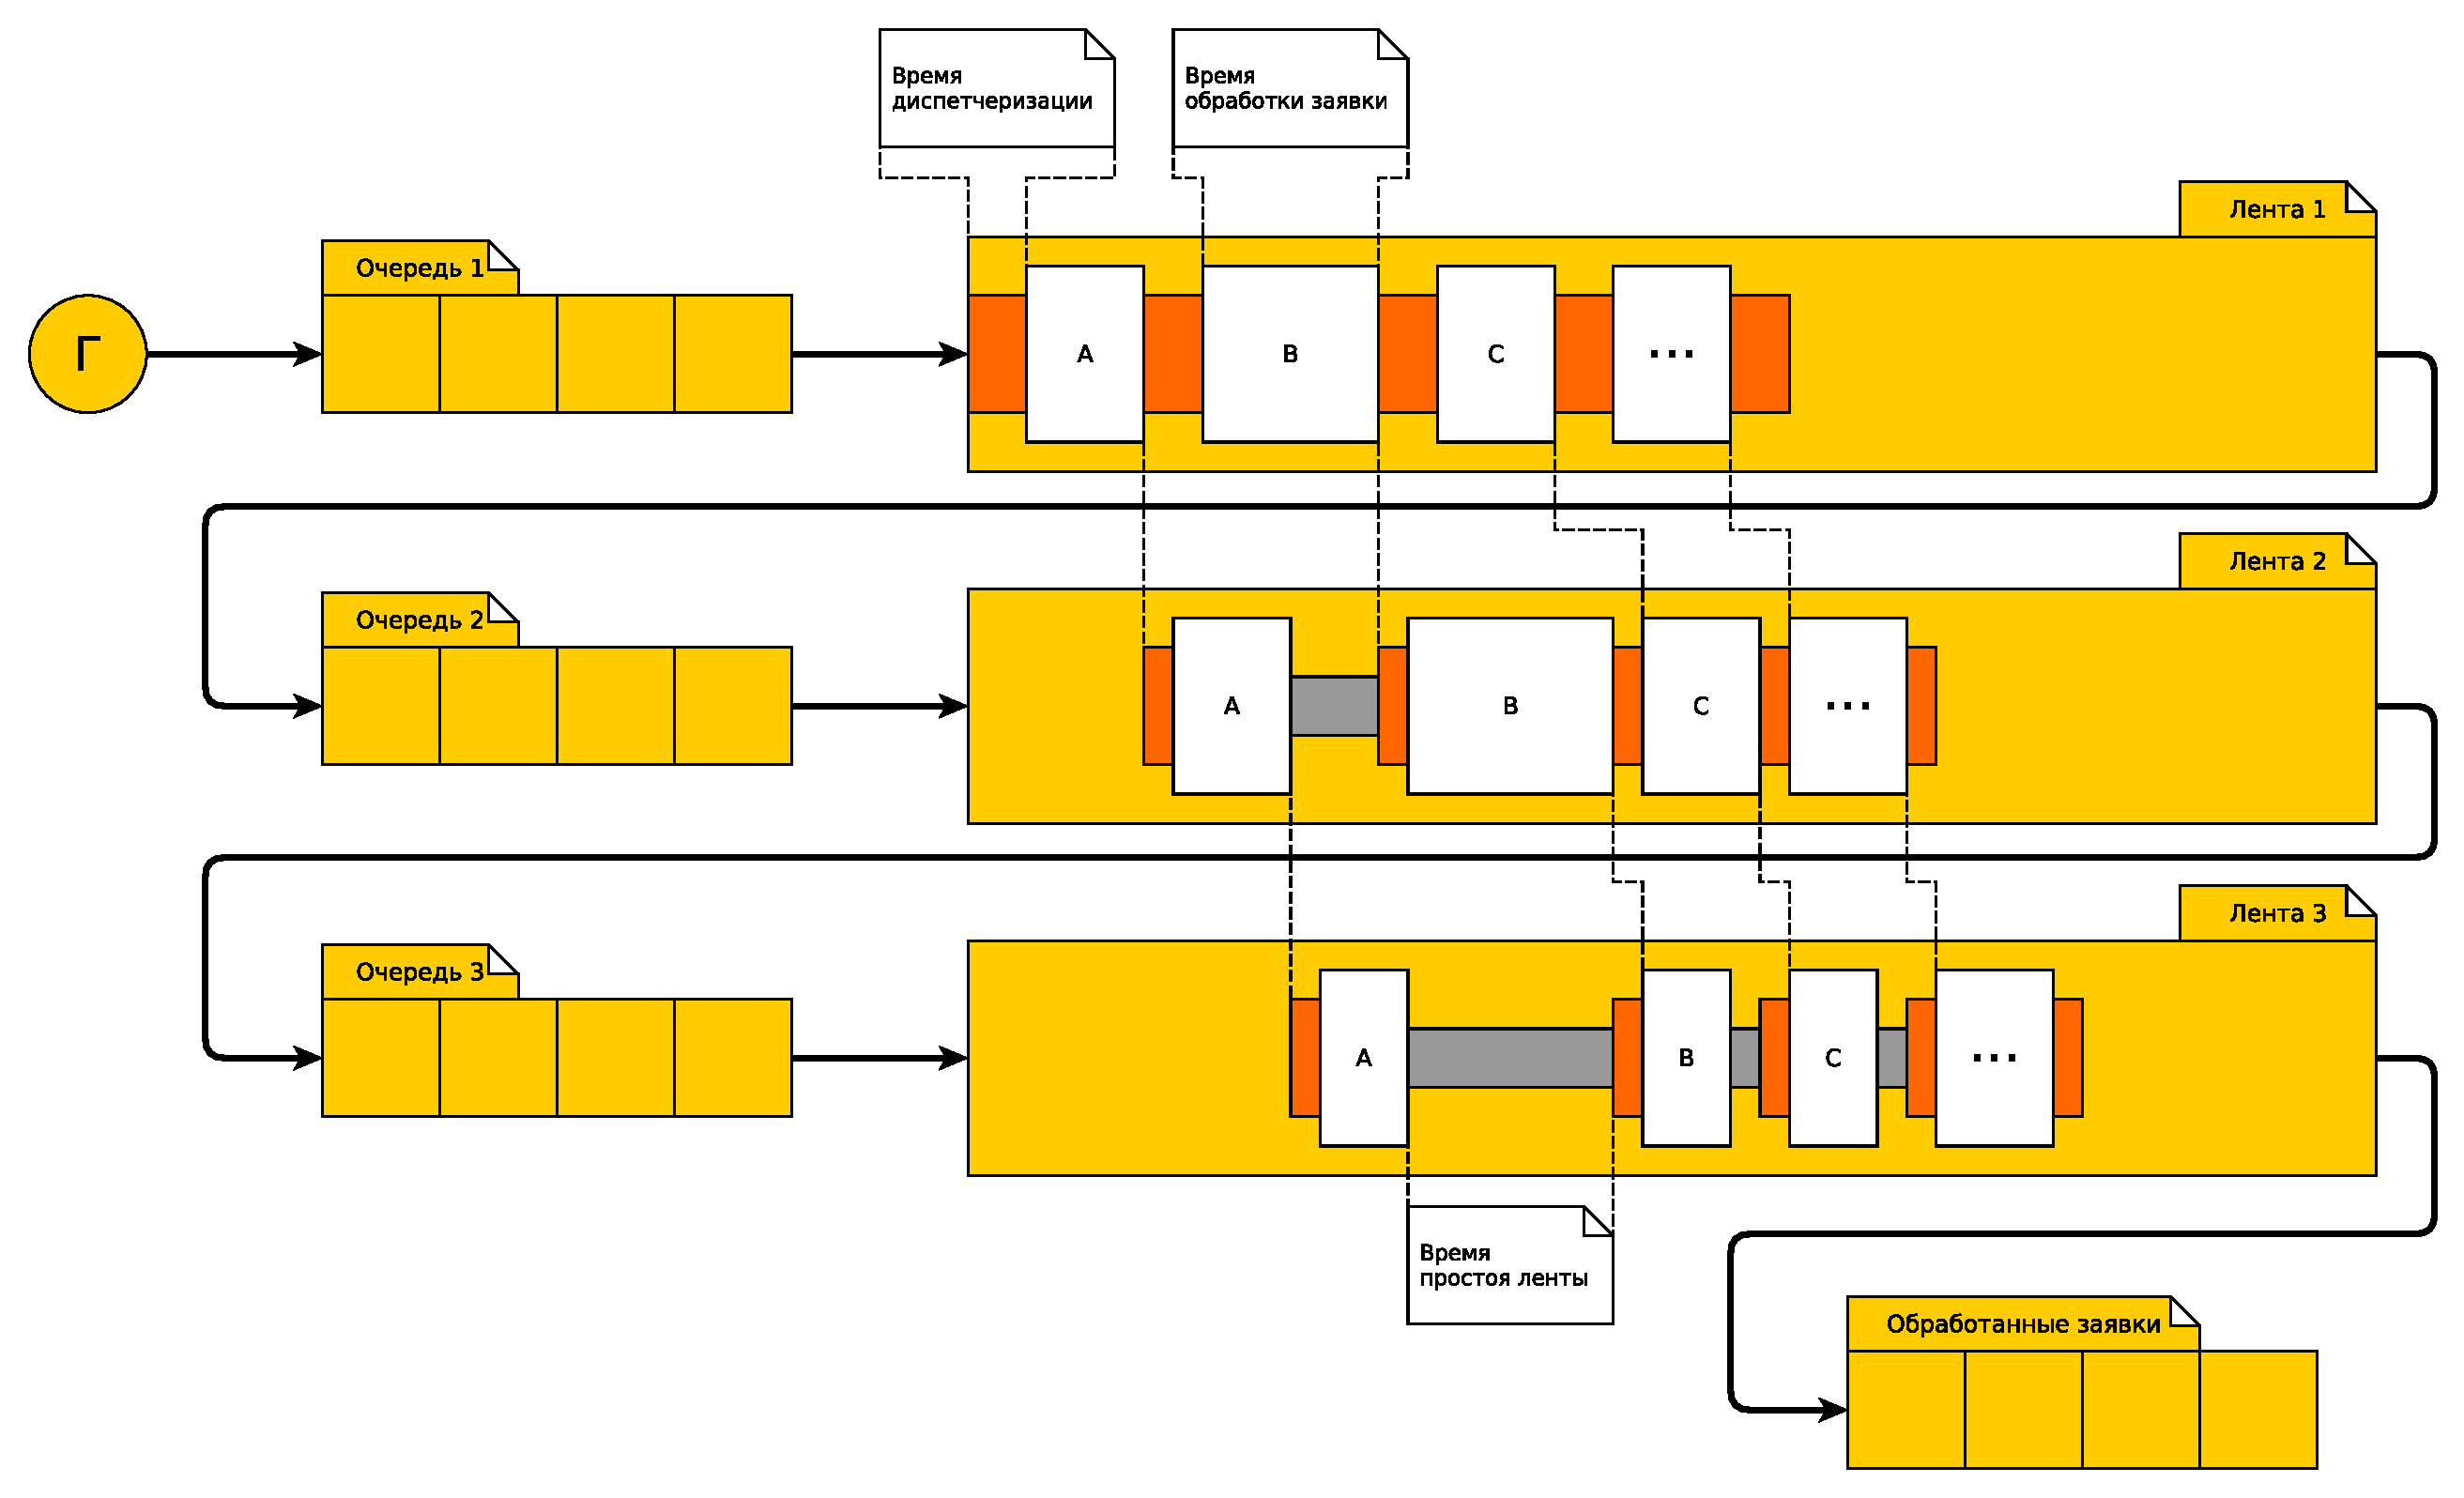
\includegraphics[width=1.00\linewidth]{images/conveer}
	\caption{Схема организации конвейера с тремя лентами}
	\label{img:conveer}
\end{figure}

\section{Структуры данных}
Для удобства работы были выделены следующие классы:
\begin{enumerate}
	\item UserStats
	\begin{itemize}
		\item поля
		\begin{itemize}
			\item times - массив из объектов класса Times, содержащий время поступления и выхода для каждой ленты конвейера;
			\item user - объект класса User, содержащий данные пользователя;
			\item current - хэш-значение пароля;
			\item number - идентификатор объекта класса;
		\end{itemize}
		\item методы
		\begin{itemize}
			\item set\_time - установка времени входа/выхода для конкретной ленты;
			\item get\_time - получение времени входа/выхода для конкретной ленты;
		\end{itemize}
	\end{itemize}
	\item User
	\begin{itemize}
		\item поля
		\begin{itemize}
			\item login - логин пользователя;
			\item password - пароль пользователя;
		\end{itemize}
		\item методы
		\begin{itemize}
			\item generate\_pass - генерирует случайный пароль;
		\end{itemize}
	\end{itemize}
	\item Time
	\begin{itemize}
		\item поля
		\begin{itemize}
			\item time\_in - время поступления на ленту ковейера;
			\item time\_out - время выхода с ленты конвейера;
		\end{itemize}
		\item методы
		\begin{itemize}
			\item set - установка времени поступления/выхода;
			\item get - получение времени поступления/выхода;
		\end{itemize}
	\end{itemize}
\end{enumerate}

Таким образом, программа генерирует заданное в программе количество пользователей и их данных, затем формирует 4 очереди и 3 ленты конвейера и запускает конвейерную обработку. После окончания выводится время конвейерной и последовательной обработки одних и тех же данных, после выводится лог, содержащий время поступления в очередь и выхода задач для каждой ленты конвейера.

\section*{Вывод}
В данном разделе приведена схема работы конвейера, выделены структуры данных для реализации в технологическим разделе. 

\end{document}
